\documentclass{arduino}
\usepackage{lipsum}
\setmainlanguage{english}
\graphicspath{{images/}}

\begin{document}

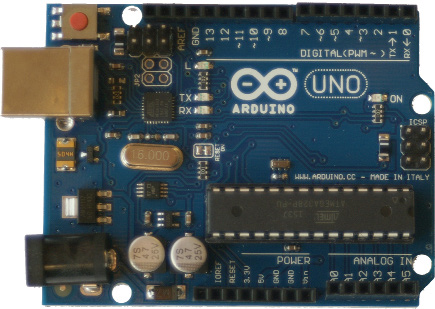
\includegraphics[width=6cm]{1. Arduino}

\textbf{Requirements for this module}

\begin{tabular}{p{0.5\textwidth}p{0.5\textwidth}}
\textbf{Offline} & \textbf{Online}\\
Arduino & --- \\
Breadboard & --- \\
Jumper cables & --- \\
Resistors (\SI{220}{\ohm}; \SI{330}{\ohm}; \SI{1}{\kilo\ohm}; \SI{10}{\kilo\ohm}) & --- \\
Potentiometer (\SI{1}{\kilo\ohm}; \SI{10}{\kilo\ohm}) & --- \\
Diode & --- \\
2x LDR & --- \\
LED (red, yellow, green) & --- \\
RGB LED & --- \\
Servo motor & --- \\
DC Motor & --- \\
5x Push button & --- \\
2N2222 transistor & --- \\
LCD & --- \\
Active piezo element & --- \\
\end{tabular}

\textbf{Prerequisite knowledge}

\begin{tabular}{ll}
Ohm's law & $R = \dfrac{U}{I}$\\
Components in series & equal current \\
Components in parrallel & equal voltage \\
Power & $P = U \cdot I = I^2 \cdot R$ \\
\multicolumn{2}{l}{Alternator / electric motor operation}\\
\end{tabular}

\newpage

\section{Introduction}

\marginfigure[\baselineskip]{2. Aurduino - welcome}
Nice that you are getting started with Arduino! Perhaps you have no idea what an Arduino is and what you can do with it. An Arduino is a kind of microcomputer. You can connect the Arduino to a computer from where you send a program (in Arduino they call it a sketch) to the Arduino. The Arduino will then run your written script and take care of the output. For example, you can keep a refrigerator at a certain temperature, control a self-driving robot, make light sensors, control an LCD screen on your shirt and so on. It is also possible not to use software and only play with the electronics. The Arduino is then the voltage source.

In this module we will work with the Arduino and learn the basic capabilities of an Arduino. When working with an Arduino you have two important parts: the Arduino and a breadboard. The Arduino is the computer, with input and output capabilities. You connect the electronics that are controlled by the Arduino to the breadboard.

\subsection{Breadboard}

\marginfigure[\baselineskip]{3. Arduino - breadboard}
\marginfigure[\baselineskip][0.5]{4. Breadboard}
The breadboard has two columns on both sides that are connected to the power supply (+ and -). The + side is connected to the \SI{5}{\volt} output or to an output port of the Arduino. The - side is connected to the GND (ground) of the Arduino. Although you do not always use the constant output, it is wise to always connect it.

The breadboard has rows and columns. The figure to the right shows a breadboard, and below it you see how the connections are made internally. The points in a row are connected. But let's not dwell on this too long\dots let's get started!

\textbf{NOTE:} Often you have to indicate to which USB port your Arduino is connected to your computer. You do this by going in the program to: Tools / Port. There you can click on the correct USB port.

\newpage

\subsection{Assignment 1 Connecting an LED}

\marginpar{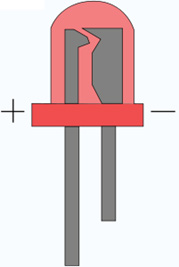
\includegraphics[width=0.3\linewidth]{5. Component LED}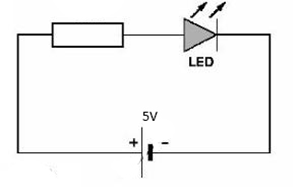
\includegraphics[width=0.7\linewidth]{6. LED circuit}}
An LED is a diode that emits light when current flows through the LED. The LED only allows current to flow in one direction. The long leg of the LED must always be connected to the + side, the short leg to the - side, see the figure on the side.

The current through an LED can usually only be \SI{20}{\milli\ampere}. The voltage across the LED is then approximately \SI{2.0}{\volt}, these values ​​differ a bit per type of LED, see table below. The Arduino supplies a \SI{5.0}{\volt} voltage. The LED must therefore be connected in series with a resistor. The resistance must therefore be at least \SI{150}{\ohm} ($R = \frac{U}{I} = \frac{\SI{3.0}{\volt}}{\SI{0.020}{\ampere}} = \SI{150}{\ohm}$).


\marginfigure[\baselineskip]{8. Circuit switchable LED}
\begin{enumerate}
\item There is no resistor with \SI{150}{\ohm}, but there is one of \SI{220}{\ohm}. Look up the resistor with the help of the color code: the first ring must be red, the second ring also and the third ring brown ($\textcolor{red}{2}\textcolor{red}{2} \cdot \textcolor{brown}{10}$). Another possibility is red, red, black, black ($\textcolor{red}{2}\textcolor{red}{2}\textcolor{black}{0} \cdot \textcolor{black}{1}$).

\item Now connect the \SI{5}{\volt} output of the Arduino to the + column and the GND (ground) output of the Arduino to the - column.

\item Connect the LED and the resistor in series, see the drawing.

\item Connect the Arduino to the computer via the USB. If you did it correctly, the LED will light!
\end{enumerate}

Because the red LED emits light at a lower voltage than, for example, a green LED, you can use a smaller resistance for green and blue LEDs. In this way they burn just as brightly!

\begin{tabular}{ll}
\textbf{Colour} & \textbf{Threshold voltage}\\
Blue & \SI{2.3}{\volt} \\ 
Green & \SI{2.0}{\volt} \\
Red  & \SI{1.5}{\volt} \\
\end{tabular}

\begin{minipage}[t]{\linewidth}
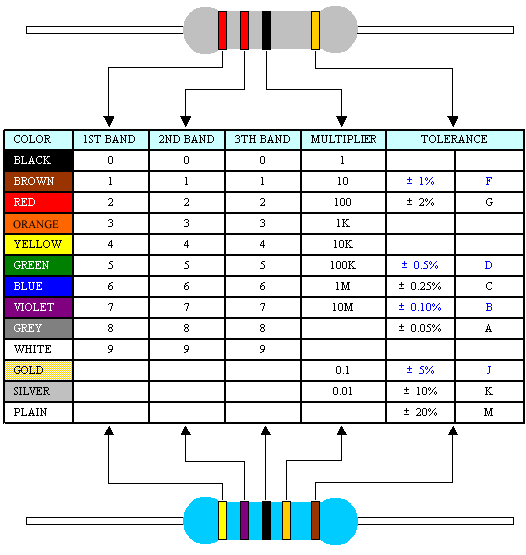
\includegraphics[width=0.8\linewidth]{7. Component resistor values (EN)}
\end{minipage}

\newpage
\subsection{Assignment 2 A blinking LED}

\marginfigure[\baselineskip]{9. Circuit blinking LED}
\marginfigure[\baselineskip]{8. Circuit switchable LED}

Now you can light your LED, but that won't be of much use to you yet\dots The next step is to control the LED using a piece of code. To control the LED using code you need to connect an output port (for example pin 13) of the Arduino to your LED. You don't need the \SI{5}{\volt} output now, pin 13 now supplies the voltage. In the drawing you can see that the \SI{5}{\volt} output is still connected. With larger projects you quickly forget the \SI{5}{\volt}, that's why it's smart to always connect it!

\begin{enumerate}[label={\alph*})]
\item Build the setup you see in the drawing and connect the Arduino to the computer.
\end{enumerate}

We want to control the Arduino, we use the Arduino program for that.

\begin{enumerate}[label={\alph*})]
\item Open the program and open the script blink via: file / examples / base / blink.

\item Check the script with the check mark. If the program does not work, it will display an error message at the bottom (you may have to assign the COM port, you do this via tools / port).

\item Upload the script to your Arduino using the button 
\includegraphics{10. Arduino upload} (shortcut: ctrl + u)

\item Briefly describe what you see. Try to explain what you see using the code.

\item Change the script so that the LED flashes faster.

\item Connect three different LED lights, change the script so that they turn on sequentially.

\item Change the script and create a traffic light with orange on for a short time.
\end{enumerate}

\newpage

\newlength{\biggraphicwithtext}
\setlength{\biggraphicwithtext}{\dimexpr(\textwidth+65mm)\relax}
\newlength{\textwidthnexttobiggraphic}
\setlength{\textwidthnexttobiggraphic}{\dimexpr(\biggraphicwithtext-120mm)\relax}
% \newlength{\biggraphic}
% \setlength{\biggraphic}{\dimexpr(\biggraphicwithtext-10mm)\relax}
\begin{minipage}{\biggraphicwithtext}
\begin{minipage}{\textwidthnexttobiggraphic}
\section{Programming part 1}\vspace{\baselineskip}

Arduino has its own programming language based on C++. If you already have experience with programming and/or with C++ (or Java), programming is very easy. And if you have no experience with programming? It's much less difficult than you might think! \vspace{\baselineskip}

At the top of the script Blink the first character is /*, which means that everything after this starting character and before the closing character */ is commented out. The code in between these characters is ignored by the program. Here you put the name of the program, what it does, who made it and when you last changed it.
\end{minipage}\hfill\begin{minipage}{12cm}
\raggedleft
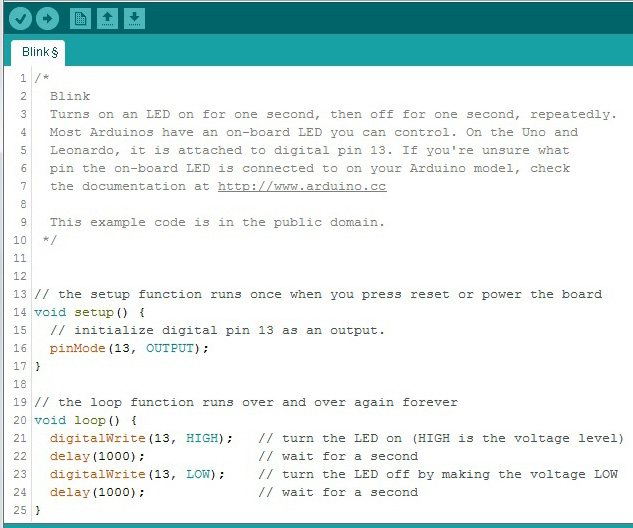
\includegraphics[width=11cm]{12. Arduino code}
\end{minipage}
\end{minipage}

\smallskip

A second possibility to add comments is with the help of //. Everything on the same line after // is a comment. This way you can keep track of what the code does on that line. With the help of the shortcut ctrl+/ you can quickly comment out an entire line of code.
\begin{marginlisting}
void setup(){
  pinMode(13,OUTPUT);
}
\end{marginlisting}

Before the most important code is executed, you must say what exactly is being controlled. First we tell the Arduino that there is something on pin 13 and that the Arduino should give an output (voltage). It would be a bit neater to first define the name of pin 13 before setup: you give the pin a name (\lstinline{int LEDred = 13;}). If you then want to control pin 13, you can do that with the name LEDred.
\begin{marginlisting}
void loop() {
  digitalWrite(13, HIGH);
  delay(1000);
  digitalWrite(13, LOW);
  delay(1000);
}
\end{marginlisting}

Everything in between the curly brackets \{\} of the loop is repeated continuously. First pin 13 is made high (\SI{5.0}{\volt}) using the code \lstinline{digitalWrite} (\lstinline{digitalWrite} can only be on or off). Then the program must wait \SI{1000}{\milli\s} before executing the next line of code. The next line of code makes pin 13 low again (\SI{0.0}{\volt}). Then the program must wait \SI{1000}{\milli\s} again, before it starts the loop again.

\marginfigure[-3\baselineskip]{13. PWM}

The pin is controlled with a high or a low signal. Is there anything else in between? Yes and no \dots The output is always \SI{0.0}{\volt} or \SI{5.0}{\volt}. But you can dim the LED by only turning on the LED for a certain time. If the LED flashes fast enough, you will not see the LED flashing, it just seems that the LED is less bright. If you want to dim an LED, use an output with the symbol $\sim$. This is a Pulse Width Modulation (PWM). The value of the PWM is between 0 (fully off) and 255 (fully on).
\newpage

\subsection{Assignment 3 A dimmable LED}

\marginfigure[\baselineskip]{14. Circuit dimmable LED}

\begin{enumerate}[label={\alph*})]
\item Build the setup on the right. Use a PWM pin for the output, for example Pin 9 (note, the LED does not need to be connected to the constant voltage, the voltage is now supplied by pin 9).

\item Open the script Fade in the examples / base and upload the script.

\item Describe what you see and try to explain what is happening with the help of the code.

\item Change the code so that the LED lights up faster and is off faster. Note, there are two ways! Try them both.

\item \lstinline{analogWrite} is used in the code. Previously we used \lstinline{digitalWrite}. Explain why this is not possible now.
\end{enumerate}

\subsection{Assignment 4 An on and off button for the LED}

\marginfigure[\baselineskip]{15. Circuit LED button}

We can now turn the LED on and off with the help of the code and even dim it. But often you also want to be able to switch a circuit on and off manually. We need a push button for that.

\begin{enumerate}[label={\alph*})]
\item Build the circuit on the right. Make sure you use a large resistor so that the supplied current is limited, because an Arduino is bad at supplying large currents.
\end{enumerate}

The idea is now that we use pin 2 as INPUT. Pin 2 measures the voltage at that point (compares it with \SI{0.0}{\volt}). This is done with the code \lstinline{digitalRead()}. It can now measure a high (\SI{5.0}{\volt}) or low (\SI{0.0}{\volt}) signal. With an analog pin such as A0 to A5, intermediate volages can also be measured, with 10-bit resolution. Pin 2 should only measure a voltage when the button is pressed.

\begin{enumerate}[label={\alph*})]
\item Open the Button script via examples / digital and upload the script.

\item Press the button and check when the LED is off and when it is on.

\item Adjust the script so that the function of the button is reversed.
\end{enumerate}

\marginfigure[-\baselineskip]{16. Button bounce}

\textbf{NOTE:} There is something special going on with the button. A button posses so-called Bounce. This means that the voltage does not go directly from \SI{0}{\volt} to \SI{5}{\volt} but goes up and down again. This is because there is a spring in the button that goes up and down. When using and reading the button it is therefore useful to build in a delay\dots

\newpage

\section{Programming part 2}

The Button script is more comprehensive than we've seen before. We walk through the script step by step.

\begin{marginlisting}
const int buttonPin = 2;
const int ledPin = 13;
\end{marginlisting}

We are dealing with two pins on the Arduino where something has to be done. Pin 2 is an input and pin 13 must be an output. The pin does not change, it is a constant (\lstinline{const}). It is an integer value (\lstinline{int}). We give pin 2 a recognizable name, pin 2 is now called buttonPin. Pin 13 has been named ledPin.

\begin{marginlisting}
int buttonState = 0;
\end{marginlisting}

We will soon want to know what the "state" of the button is (pressed or not). It can be 1 or 0. First we have to tell the Arduino that we want to later know the state of the button (create a variable). Before we run the script, the buttonState equals 0.

\begin{marginlisting}
void setup() {
  pinMode(ledPin, OUTPUT);
  pinMode(buttonPin, INPUT);
}
\end{marginlisting}

As mentioned, we have to tell you that the ledPin is an \lstinline{OUTPUT} and the buttonPin is a \lstinline{INPUT}. Now the Arduino knows that too\dots

But something must happen when the button is pressed. At the start of the loop, the button is read (actually the voltage across the resistor is measured to see if it reads \SI{5.0}{\volt}). Subsequently an \lstinline{if} statement follows. If (\lstinline{if}) the button is pressed (\lstinline{buttonState == HIGH}) then the LED should light (\lstinline{digitalWrite (ledPin, HIGH);}). In all other cases (\lstinline{else}), the LED should not be lit (\lstinline{digitalWrite (ledPin, LOW);}).

\begin{marginlisting}
void loop() {
  buttonState = digitalRead(buttonPin);
  if (buttonState == HIGH) {
    digitalWrite(ledPin, HIGH);
  }
  else {
    digitalWrite(ledPin, LOW);
  }
}
\end{marginlisting}

It's an easy \lstinline{if} statement. You can also set multiple conditions. If you have to press two buttons at the same time before the LED turns on, put \lstinline{&&} between the characters (\lstinline{if buttonState1 == HIGH && buttonState 2 == HIGH)}).

You can also use the character \lstinline{||}. Then either one condition must apply or the other. Unfortunately, the light does not yet stay on when you have pressed the button. But you can change the code to make sure that the light can be switched on and off with one button.

\begin{marginlisting}
void loop() {
  buttonState = digitalRead(buttonPin);
  if (buttonState == HIGH && state == LOW) {
    state2 = HIGH;
    }
  if (buttonState == HIGH && state == HIGH) {
    state2 = LOW;
    }
  state = state2;
  digitalWrite(ledPin,state);
  delay (100);
}
\end{marginlisting}

\begin{marginlisting}
if(buttonState == HIGH){i++;}
digitalWrite(ledPin,i%2);
\end{marginlisting}
Don't forget to define the new variable (\lstinline{int}) at the beginning! There are even simpler ways, these are only shown as script. Explain how they work!

\begin{marginlisting}
digitalWrite(13,!digitalRead(13));
\end{marginlisting}

\newpage

\subsection{Assignment 5 Securing a safe}

The bank's safe is secured. The safe does not open (the LED will only light up) when two keys are turned (buttons pressed). One keyhole is in the warden's room, the other is next to the safe.

Build the corresponding circuit and program the script so that the safe does not open until both keys are turned at the same time.

\subsection{Assignment 6 A two-way switch}

When you are at the bottom of the stairs you want to turn on the light at the top of the stairs. There is another light switch at the top of the stairs. With that you can turn the light off or on again. Build the circuit with two buttons and write the program so that you have a working two-way circuit. Does this not work immediately? Then try it first with a single button.

\subsection{Assignment 7 A pedestrian crossing}

A special transition area has been created for pedestrians. This place is on a busy road. If there are no pedestrians, the traffic light in front of the cars is green. The moment a pedestrian wants to cross, he presses the button. The traffic light in front of the cars then changes from green to yellow to red. Pedestrians then have 15 seconds to cross. The traffic light in front of them is green! Then the green light will blink five times and change to red. A second later, the traffic light in front of the cars turns green again.

Make this system.

\newpage

\section{Electronics part 1}

\marginfigure[0pt][0.7]{17. Component LDR}

\marginfigure{18. LDR resistance vs light intensity}

With only a button and an LED you can quickly become bored, and we have hardly scratched the surface of what an Arduino can do\dots We want to control robots, prevent collisions of racing cars with walls, or to automatically control greenhouses, and so on. In order to achieve that we need sensors. Almost all sensors work the same, the resistance value changes with a changing input (for example light or force). We are going to start with a light sensor. For a light sensor we need an LDR, see the photo. LDR stands for Light Dependent Resistor. The resistance value changes with changing light intensity, see the graph.

\marginfigure[0pt][0.7]{19. LDR circuit}

We connect the LDR in series with an ohmic resistor (a resistor with a constant resistance value). This way we can create a voltage divider. Part of the voltage is across the LDR and part of the voltage is across the resistor. All we have to do is read the voltage across the LDR and we know how how much light shines on the LDR!

It is important to know a little more about how a voltage divider works. The LDR and the ohmic resistor are in series so that: $ R_\mathrm{total} = R_\mathrm{LDR} + R_{\si{\ohm}} $. The source voltage is \SI{5.0}{\volt}, and because the resistors are connected in series, the current is the same everywhere in the circuit.

You calculate the current with: $ I = \frac{U_\mathrm{source}}{R_\mathrm{total}} $. 

The voltage is distributed so that the largest resistance receives the largest voltage. If you combine this information you will see that the ratio between the voltages is equal to the ratio between the resistors: $ \frac{U_\mathrm{LDR}}{U _ {\si{\ohm}}} = \dfrac{R_\mathrm{LDR}}{R_{\si{\ohm}}} $.

\marginfigure{20. LDR potantial vs resistance}

When the LDR picks up more light, the resistance value of the LDR decreases: there will be a lower voltage across the LDR but a higher voltage across the ohmic resistor. The voltage across the LDR ($ U_\mathrm{LDR} = \SI{5.0}{\volt} \cdot \dfrac{R_\mathrm{LDR}}{(R_\mathrm{LDR} + R_{\si{\ohm}})} $ can be measured using the ANALOG IN of the Arduino, so that the voltage is then a measure of the measured light intensity.

Depending over which range your sensor should be sensitive determines the choice of an ohmic resistor. See the second graph. The LDR has a value between \SI{10}{\kilo\ohm} and \SI{20}{\kilo\ohm}: so choose a large resistor!

\newpage

\subsection{Assignment 8 A light sensor}

\marginfigure{21. Circuit light sensor}

The circuit is very similar to Assignment 4. Only now we use an LDR and an ANALOG IN.

\begin{enumerate}[label={\alph*})]
\item Build the circuit.

\item Open the analogReadSerial  script: examples / base / Analogreadserial.
\end{enumerate}

The most important code can be found below.

\begin{lstlisting}
void loop() {
  int sensorValue = analogRead(A0);
  Serial.println(sensorValue);
  delay(10);
}
\end{lstlisting}

The Arduino is instructed to read out the analog port (\lstinline{analogRead (A0)}). This value is linked to the variable \lstinline{sensorValue}. 

Next we want to know this value. The value is then also printed for us (\lstinline{Serial.println (sensorValue);}), which can be read using the serial monitor (the magnifying glass at the top right). For stability it is good to build in a \lstinline{delay}.

\begin{enumerate}[label={\alph*})]
\item Upload the script to the Arduino and read the values ​​using the Serial Monitor.

\item Cover the LDR with your hand. Does the given value change?

\item Combine assignment 3 and this assignment. Make sure the LED lights up brighter when it gets darker.

\item Expand the circuit further so that you can switch the entire circuit on and off with a button.

\item Using graph 2, explain that a large value of $ R_{\si{\ohm}} $ makes the LDR almost equally sensitive throughout the range.

\item Think of a way to calibrate the sensor yourself. So let the sensor itself determine the minimum and maximum value.
\end{enumerate}


\subsection{Assignment 9 Measure response time}

Build a response timer that requires someone to press the button as soon as possible when a red LED goes out and a green LED comes on. To make this more difficult for the person who has to press the button, you can use function \lstinline{random (a, b)}. In which \lstinline{a} and \lstinline{b} are numbers, so using this function you can build in a random delay. The function \lstinline{millis()} defines how many milliseconds have passed.

\newpage

\section{Programming part 3}

\marginfigure[-\baselineskip]{22. Arduino mapping}

The Arduino cannot read all values. The ANALOG IN has a 10 bit chip. This means that the resolution is limited to $ 2^{10} = 1024 $ values. It's like dividing the \SI{5.0}{\volt} into 1024 small blocks. The value that you read out at task 8 is therefore not the voltage itself, but the number that belongs to a voltage. So the number 223 belongs to: $ \dfrac{223}{1023} \cdot \SI{5.0}{\volt} = \SI{1.09}{\volt} $. The PWM ($\sim$) is an 8 bit system and can therefore give $ 2^8 = 256 $ values.

Oops \dots do you see the problem? We can read with 1023 different values, but writing is only possible with 255 values ​​\dots. Fortunately, there is a code that provides automatic scaling (\lstinline{map}).

\begin{marginlisting}
void loop() {
  sensorValue = analogRead(sensorPin);
  brightness = map(sensorValue,500,900,255,0);
  Serial.println(sensorValue);
  delay(10);
  analogWrite(ledPin,brightness);
}
\end{marginlisting}
The \lstinline{map} function requires 5 numbers for information. The first number is the value that the analog port reads. The second number is the lowest number that can be read, the third number is the largest value that can be read. This does not necessarily have to be 0 and 1023, you get the value when calibrating your sensor. The sensitivity of your sensor can therefore also be between 500 and 900, see again graph 2 from programming part 3. The fourth and fifth numbers indicate the range of the output. In the example, an input value of 500 should become an output value of 255. An input value of 900 should become an output value of 0.

\begin{marginlisting}
void loop(){
  for(i<5;i++;) {
    digitalWrite(LEDPin,HIGH);
    delay(100-i);
    digitalWrite(LEDPin,LOW);
    delay(100);
  }
  [...]
}
\end{marginlisting}
Another useful feature is the \lstinline{++} function. Each time the loop enters the next cycle, the value is incremented by 1. For example, you can easily keep track of how many loops (iterations) there have already been. It is also possible in this way to control a different pin each time or to change a frequency later.

If \lstinline{++} exists, then \lstinline{--} will also exist. And that's right. \lstinline{--} causes the value to be decreased by 1. Both codes can be placed in a \lstinline{for} loop. This is a loop within the loop. Take a look at the example where there is some kind of countdown mechanism in it before the program itself starts\dots (note, you still have to declare the variable \lstinline{i} for the setup!

\subsection{Assignment 10 Faster programming}

Rewrite assignment 2h with the function \lstinline{++}.

\subsection{Assignment 11 Alarm switch}

Under the cash register of a shop there is a switch (push button). Once pressed, a pulsating alarm bell should ring. Mimic the function of the alarm bell by pulsing an LED. Make this system.

\newpage
\subsection{Assignment 12 An RGB LED}

\marginfigure{23. Component RGB LED}
\marginfigure{24. Component potentiometer}
\marginfigure{25. Circuit RGB LED}

An RGB LED has four legs. The LED actually contains three LEDs. By controlling the three LEDs with the help of a PWM ($\sim$) you can mix colors and get intermediate colors. Now we can determine the strength of each color through the software, but it would be nice if we could also manually set the colors. We use variable resistors also called potentiometers for this.

The potentiometer has three legs. One for the \SI{5.0}{\volt} in, one for the earth (\SI{0.0}{\volt}) and one leg for reading the meter using an analog pin. see also the figure on the right .

When you turn the rotary knob of the potentiometer, the resistance changes, which also changes the value of the voltage that you read out. A potentiometer is actually a voltage divider.

\begin{enumerate}[label={\alph*})]
\item Build the circuit.

\item Write the corresponding code, first reading out the value of the potentiometer and then controlling the RGB LED.

\item Try the different positions of the RGB LED and check if the picture below corresponds well with the colors of the LED.
\end{enumerate}

\begin{center}

\includegraphics[width=5cm]{26. Mixing colours}
\end{center}

\newpage

\subsection{Question 13 The speed of an electric motor}

\marginfigure[0pt][0.7]{27. Component motor}

\marginfigure[0pt][0.7]{28. Component motor schematic}

An electric motor converts electrical energy into kinetic energy. You will find an electric motor in all devices that move and work on electricity. The speed of an electric motor depends on the voltage across the motor. In this lesson we will work with the PWM pin ($\sim$). We can of course directly enter the speed of the electric motor in our script, but it would be more convenient if we could adjust the speed of the electric motor manually, for example using a rotary knob. We are going to use a variable resistor, also called a potentiometer.

\begin{enumerate}[label={\alph*})]
\item Build the right side of the circuit with the potentiometer. You don't have to connect the electric motor yet.

\item Explain why the signal out of the potentiometer should go to ANALOG IN.

\item Explain why the diode is included in the circuit.

\item Program the accompanying script so that the speed of rotation of the electric motor can be set using the potentiometer. Use the map function for this.
\end{enumerate}

\begin{center}
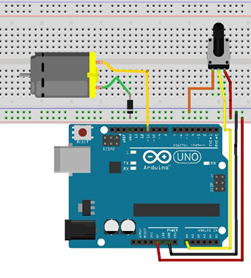
\includegraphics[width=0.8\textwidth]{29. Circuit motor control}
\end{center}

\newpage

\section{Electronics part 2}

\marginfigure{30. Component transistor}

\marginfigure{31. Component transistor pinout}

\marginfigure[0pt][0.8]{32. Component transistor function}

An electric motor can consume a lot of power. The Arduino is bad at providing a lot of power. To provide large power consumers with the necessary power, you can use an external power source such as a battery. Then you still need a transistor so that you can control the magnitude of the current and adjust the speed of rotation of the electric motor.

The transistor (here we only use a so-called NPN transistor) has three legs, see the photo. The emitter is on the left, the base in the middle and the collector on the right. (ATTENTION! With several transistors the pin order is different, we assume you use the 2N222 transistor). The external power supply (+ side) is connected to the collector at all times. Voltage across the base determines whether current will flow to the emitter. This makes a transistor a kind of tap: the amount of voltage at the base determines the amount of current that is passed. The base must therefore be controlled with a PWM pin if you want to control the speed.

With very high currents you have to use a larger transistor or one with a cooling element so that the transistor can lose its heat.

\subsection{Question 14 The speed of an electric motor part 2}

The circuit of assignment 13 is too simple and the Arduino may well be supplying too little current. Especially when you want to run the DC motor quickly.

\begin{enumerate}[label={\alph*})]
\item Build the circuit as shown below.

\item Use the script from assignment 12 and upload the program. Can the electric motor actually turn faster?
\end{enumerate}

\begin{center}
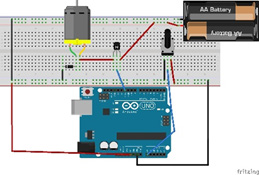
\includegraphics[width=0.8\linewidth]{33. Circuit motor control (large current)}
\end{center}

\newpage

\section{Programming part 4}

\marginfigure[\baselineskip][0.5]{34. Component servo}

Scripts have already been written for controlling some devices, making controlling the devices easier. One of those devices is a servo motor. A servo motor is a type of electric motor that can rotate \ang{180}. The rotation angle can be set precisely because it works with a built-in potentiometer. To use a servo we need the following script.

\begin{lstlisting}
#include <Servo.h>
Servo mijnServo;
int pos = 0;
void setup() {
  mijnServo.attach(9)
}
\end{lstlisting}

First, the script is retrieved from the library. Then we call the servo myServo and it gets the starting position 0.

With \lstinline{myServo.attach (9)} we say that the servo is connected to pin 9. Of course this is another PWM port.

Now it is possible to control the servo. Where pos stands for the position, it can be between 0 and 180. The code for controlling this servo will then be: \lstinline{myServo.write (pos);} A servo motor cannot rotate completely like a normal electric motor, but we can aim very well with a servo motor. This is because there is a potentiometer in the Servo, so the control is done by reading the voltage!

\subsection{Assignment 15 A light measuring device}

Use assignment 8 as a basis. Replace the LED with the servo motor. You can stick a pointer on the servo and make a scale so that the pointer indicates how light / dark it is.

\subsection{Question 16 As much sunlight as possible}

\marginfigure{35. Control light}

Solar panels are installed to convert radiant energy from the sun into electrical energy. The panels receive the most light when they are perpendicular to the sun. The earth rotates and we should let the panels rotate to capture as much energy as possible. We are going to do that in this assignment.

All solar panels are set up on a large field, such as solar panel 1. Solar panel 2 and 3 are both slightly rotated in relation to panel 1. You can now clearly see that the solar panels would produce the most electrical energy if solar panels 2 and 3 would produce the same amount of electrical energy. However, currently panel 2 now captures more light rays than panel 3. So the whole system should be turned counterclockwise.

\newpage

\marginfigure{36. Circuit solar panel control}
Instead of a solar cell, we start with an LDR.

\begin{enumerate}[label={\alph*})]
\item Build the circuit and program the first piece where you can read the values ​​of the LDR.

\item Turn on the flash of your phone and read using \lstinline{Serial.println(LDR1);} the values ​​of LDR 1 and LDR2. Move your phone from left to right and watch the values ​​vary.

\item Now write the piece of code for the servo. Turn the servo to the left if LDR1 receives more light than LDR2 and vice versa. Keep in mind that the servo uses a potentiometer and you can also use the map function.

\item Explain that it is already quite close to rotating the solar panels.
\end{enumerate}

\begin{minipage}{\widemargin}
\subsection{Assignment 17 LCD}

With an LCD screen (liquid crystal display) it is possible to print information on a small screen. This eliminates the need to use the serial monitor (and computer) to read data.\vspace{\baselineskip}

\begin{minipage}{\textwidth}
\centering
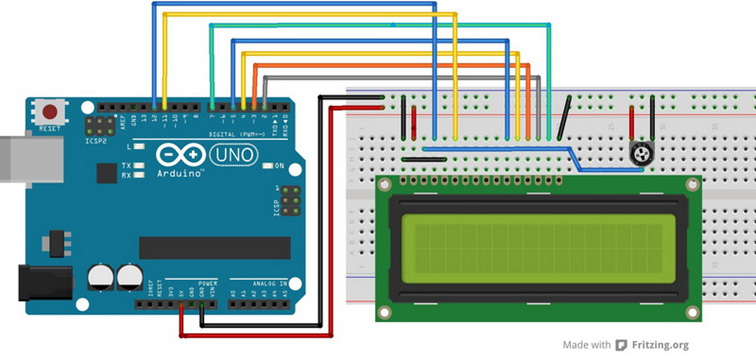
\includegraphics[width=0.7\textwidth]{37. Circuit display}
\end{minipage}

\begin{enumerate}[label={\alph*})]
\item Create the setup shown here.

\item Open the program HelloWorld, it can be found at File / examples / LiquidCrystal and upload the program. Note! With HelloWorld your backlight is not yet on, you can control this using pin 7 (and insert the piece of code). You can also always have the backlight on by not connecting to pin 7 but to the +.

\item Try to read the script and see if you understand what the LCD shows.
\end{enumerate}

The script uses a library. A library is a piece of code written by others, which makes programming a lot easier for you. Libraries have already been made for many different sensors, so it is only a matter of finding them. This often works through, for example: \href{instructables.com}{instructables.com} or \href{arduino.cc}{arduino.cc}. All possible functions for this specific library can be found at: \href{arduino.cc/en/reference/LiquidCrystal}{https://www.arduino.cc/en/reference/LiquidCrystal}

Let's take a look at the script: after reading the library, we should specify the pins that will be used. The setup specifies that the lcd has 16 columns and two rows (\lstinline{lcd.begin(16,2);}). The text hello, world is also immediately printed (everything in the setup is done 1x!).

Over time, the time the Arduino is on (\lstinline{millis ();}) is printed to the LCD, to line 2.

\begin{enumerate}[label={\alph*})]
\item Expand your circuit with a push button and change the code so that the LCD screen shows how many times you pressed the button.
\end{enumerate}
\end{minipage}

\newpage

\section{Functions}

\begin{minipage}{\widemargin}
There is a huge list of features. What follows are the most common functions that are used in Arduino.

\begin{longtable}{p{0.22\textwidth}p{0.74\textwidth}}
\toprule
\textbf{Function} & \textbf{Explanation} \\
\midrule\endhead
\midrule \multicolumn{2}{r}{{\scriptsize\textit{Continues on the next page}}} \\ \bottomrule
\endfoot
\bottomrule
\endlastfoot 
{\lstinline[]!int!} &
value between -32768 en 32767 (215) \\
{\lstinline[]!long!} &
value between -2.147.483.648 en 2.147.483.647 (231) \\
{\lstinline[]!unsigned long!} / {\lstinline[]!unsigned int!} &
only positive values \\
{\lstinline[]!char!} &
characters stored via the ASCII system \\
{\lstinline[]!float!} &
are decimal values, but are avoided as much as possible in Arduino \\
{\lstinline[]!digitalWrite(pin,waarde);!} &
does not write voltage ({\lstinline[]!LOW!}) or a voltage of \SI{5.0}{\volt} to the pin. \\
{\lstinline[]!analogWrite(pin,waarde)!} &
Writes with an 8 bit output values ​​between 0 and \SI{5.0}{\volt}. The indicated value must be between 0 and 255. \\
{\lstinline[]!digitalRead(pin)!} &
reads if there is a voltage on the pin, returns a 0 or 1. \\
{\lstinline[]!analogRead(pin)!} &
reads how much voltage is on the pin, returns a value between 0 and 1023. \\
{\lstinline[]!map(W,Min1,Max1,Min2,Max2)!} &
Is a scaling function. Converts a value ({\lstinline[]!W!}) between {\lstinline[]!Min1!} and {\lstinline[]!Max1!} to a value between {\lstinline[]!Min2!} and {\lstinline[]!Max2!}. \\
{\lstinline[]!if(voorwaarde){}!} &
If the set condition is met, the code between the curly brackets is executed. \\
{\lstinline[]!while(voorwaarde){}!} &
As long as the condition is met, the code between the braces will be executed. \\
{\lstinline[]!for(init;cond;incr){}!} &
A for loop executes the code between the braces a number of times. {\lstinline[]!init!} is the initial value, {\lstinline[]!cond!} is the condition and {\lstinline[]!incr!} is the increment. Ex: {\lstinline[]!for(int i = 0; i<20;i++){delay(100);}!} \\
{\lstinline[]!switch case!} &
switch case is a kind of menu where a piece of code can be executed. If the variable has value one, it executes the code associated with case 1. See code block below.\\
{\lstinline[]!&&!} &
Both conditions must apply \\
{\lstinline[]!||!} &
One of the two conditions must apply \\
{\lstinline[]!!=!} &
Is not equal to. \\
{\lstinline[]!Tone(pin,f,t);!} &
Can produce specific frequency. The tone must indicate on which pin the speaker is located, which frequency must be made and possibly how long the tone must be held. It is not necessary to specify how long the tone should be held. \\
{\lstinline[]!noTone(pin);!} &
Stops the tone that was being produced. \\
{\lstinline[]!millis();!} &
This can serve as a timer. {\lstinline[]!millis();!} indicates the number of milliseconds that the Arduino is on. \\
{\lstinline[]!micros();!} &
Displays the number of microseconds that the Arduino is on. The resolution is \SI{4}{\micro\s}. \\
{\lstinline[]!delay();!} &
Wait a few milliseconds for the next piece of code to run. \\
{\lstinline[]!random(min,max)!} &
Random returns a number between the lowest value ({\lstinline[]!min!}) and highest value ({\lstinline[]!max!}). A disadvantage of random is that the same sequence is played when the Arduino is restarted. Random is not random\dots. This problem can be solved by first using the {\lstinline[]!randomSeed(analogRead(0));!} function. This reads pin A0. If nothing is connected there, noise is measured here. randomSeed shakes up Random's fixed sequence, as it were.\\
\end{longtable}
\end{minipage}

\bigskip

\begin{lstlisting}
switch (var) {
  case 1: \\ do something if var is 1
  break;
  case 2: \\ do something if var is 2
  break;
  default: \\ if neither of the above is true, then do the following (optional)
  break;
}
\end{lstlisting}

\end{document}